\documentclass[11pt,a4paper]{article}
\usepackage[utf8]{inputenc}
\usepackage[T1]{fontenc}
\usepackage{amsmath}
\usepackage{amsfonts}
\usepackage{amssymb}
\usepackage{graphicx}

\title{Notes sur l'abstraction des réseaux de neurones}
\author{Paul LANDRIER}
\date{}

\newcommand{\R}{\ensuremath{\mathbb{R}}}
\newcommand{\bb}{\mathbb}
%\newcommand{\cal}{\mathcal}


\begin{document}
\maketitle

\section{Généralité}

\subsection{Idée Générale}

On souhaite abstraire le fonctionnemet d'un réseau de neurones.

Si on appelle I le vecteur en entrée du réseau, l'exécution s'écrit naïvement :

\begin{equation}
\label{eq:eq_generale_naive}
\phi_1 ( A_1 \phi_2 (A_2 \phi_3( \dots A_{n-1} \phi_n (A_n I) \dots )))
\end{equation}

où les $(A_i)$ sont des matrices et les $(\phi_i)$ sont des fonctions d'activations, typiquement ReLU ou sigmoid coordonnée par coordonnée.

 On lui préferera en général l'écriture : 
 
\begin{equation}
\label{eq:eq_generale_transformation}
\R^{d_1} \overset{\varphi_1}{\to} \R^{d_2} \overset{\varphi_2}{\to} \dots \overset{\varphi_n}{\to} \R^{d_{n+1}}
\end{equation}

qui met plus en avant les transformtions successives, qui est le processus que l'on cherche à abstraire.

Quelques remarques :
\begin{itemize}

	\item L'équation \ref{eq:eq_generale_transformation} s'instancie en l'équation \ref{eq:eq_generale_naive} en remplaçant $\varphi_1$ par $X \mapsto \phi_n(A_n X)$, $\varphi_2$ par $X \mapsto \phi_{n-1}(A_{n-1} X)$ et plus généralement $\varphi_i$ par $X \mapsto \phi_{n-i+1}(A_{n-i+1} X)$.
	
	\item Les transformations pourront être considérées dans le sens direct (input $\to$ output), comme dans l'exemple précédent, ou indirect (output $\to$ input), comme pour la \textit{layer-wise relevant propagation}.
	
\end{itemize}

\subsection{Morphisme de variété}

	En s'inspirant de l'exemple de la provenance par semi-anneaux, nous aimerions trouver quelle structure est transportée par les applications $\varphi_i$. L'ensemble $\R^d$ est naturellement muni d'une structure d'espace vectoriel, conservée dans l'équation \ref{eq:eq_generale_naive} par la multiplication par la matrice $A_i$ mais cette structure est complètement ignorée par les activations non-linéaires, par définition. Cela nous conduit à chercher, dans un premier temps, l'abstraction de ces application d'un point de vu topologique.

	Dans \textit{Geometric Understanding of Deep Learning}, (http://arxiv.org/abs/1805.10451), Na Lei, Zhongxuan Luo, Shing-Tung Yau et David Xianfeng Gu proposent une interprétation des réseaux de neurones fondée sur les variétés.
	\\
	
	
	On aimerait ainsi de généraliser l'équation \ref{eq:eq_generale_transformation} à travers une structure topologique sous la forme :
	
	\begin{equation}
	\label{eq:variete}
V_1 \overset{\varphi_1}{\to} V_2 \overset{\varphi_2}{\to} \dots \overset{\varphi_n}{\to} V_{n+1}	
	\end{equation}

où les $V_i$ sont des variétés et les $\varphi_i$ des morphismes de variété.

Cependant, bien que les activations linéaires conservent pour la plupart la structure de variété (à l'exception notable de ReLU, elles induisent des homéomorphismes) les applications linéaires, elles, ne conservent pas cette structure. On remarque ainsi que la courbe $\{ (x,x^2), x \in \R^2 \}$, qui est une sous variété de dimension 1 de $\R^2$, est envoyée sur $\R^+$, qui n'est pas une sous variété de $\R$, par l'application $x \to <x,e_2>$ où $e_2 = (0,1)$. Dans ce premier cas, l'ensemble d'arrivée est toujours munissable d'une structure de variété à bord. Un exemple plus problématique est par exemple le cas de la variété\footnote{L'exemple a été trouvé à partir de l'échange https://math.stackexchange.com/questions/1932215/image-of-a-submanifold-under-a-linear-map et d'une discussion avec Antoine Groudiev.}
\begin{equation}
\begin{array}{l}
V = \{(\theta,r\sin(\arctan (\theta))^2,r\cos(\arctan(\theta ))^2), \theta \in  \R^-, r \in \R \} \\
\cup \ \{(\theta,0,r), \theta \in [0,1], r \in \R \} \\
\cup \ \{(\theta,r\sin(\arctan (\theta - 1))^2,r\cos(\arctan(\theta - 1))^2), \theta \in  \R^+, r \in \R \}.
\end{array}
\end{equation}

Cet ensemble est une variété différentielle et il est representé en figure \ref{fig:variete_ex}.

En revanhce, sa projection orthogonale sur le plan $(x,y)$ est $\R_{<0} \times \R \cup [0,1] \times \{0\} \cup \R_{>1} \times \R$ représenté en figure \ref{fig:variete_proj}.
\\

On a ainsi exhibé un exemple de variété dont la structure ne serait pas préservée par les transformations faites par un réseau de neurones.


\begin{figure}
	\centering
	\label{fig:variete_ex}
	\caption{La variété $V$.}
	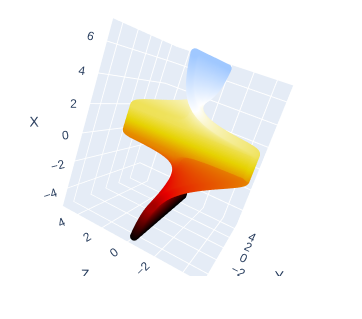
\includegraphics[scale=0.5]{manifold_ex.png}
\end{figure}

\begin{figure}
	\centering
	\label{fig:variete_proj}
	\caption{Projection orhtogonale de $V$ sur le plan $(x,y)$}
	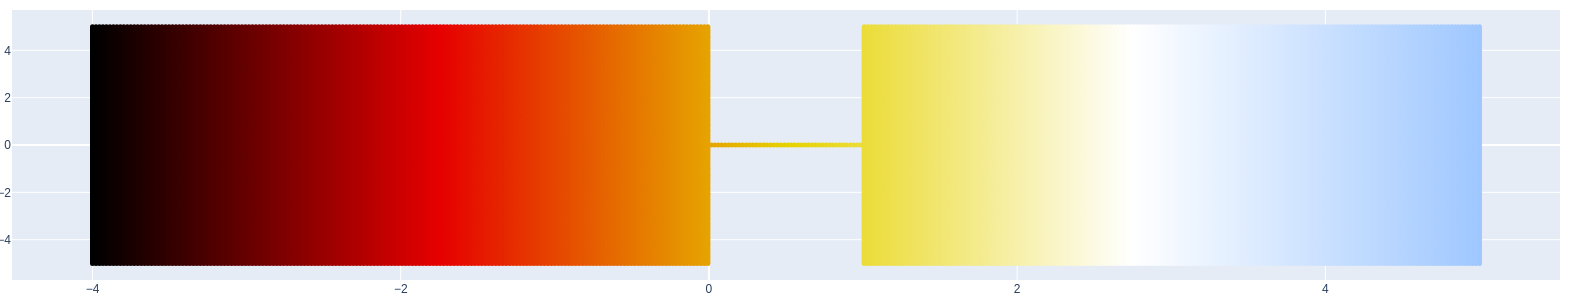
\includegraphics[width=150pt, height=150pt]{projected_manifold.png}
\end{figure}


\end{document}